\chapter{합성 보손, 스핀 표현과 디랙 이중화}

\section{교환 대칭성과 합성 보손}

첫 질문은 합성 입자를 둘러싼 실제 역설이다. 페르미온 두 개가 보손을 이룬다면, 그런 보손 두 개가 페르미온의 배타 원리를 어기지 않고 같은 상태를 차지할 수 있을까? 답은 교환 규칙 자체에서 출발한다.

두 입자를 두 인수로 표현하는 파동함수로 기술한다고 하자. 기호 \(x\)와 \(y\)는 두 입자 자리를 나타내며, 서로 다른 두 종류의 입자를 구별하는 기호가 아니다. 보손의 파동함수는 대칭이고 페르미온의 파동함수는 반대칭이다:
\begin{equation}
\Psi_B(x,y)=\Psi_B(y,x),
\qquad
\Psi_F(x,y)=-\Psi_F(y,x).
\end{equation}
이 대칭성은 구별할 수 없는 두 입자를 서로 바꾸어도 새로운 물리적 상태가 생기지 않는다는 뜻이다.

보손 두 개는 같은 단일 입자 상태를 차지할 수 있다. 그 상태의 파동함수가 \(\varphi\)라면, 두 입자의 곱은 다음과 같다.
\begin{equation}
\Psi(x,y)=\varphi(x)\varphi(y).
\end{equation}
파동함수는 연산자나 행렬이 아니라 보통의 복소수값 함수이므로 함수값은 서로 교환된다.
\begin{equation}
\varphi(x)\varphi(y)=\varphi(y)\varphi(x).
\end{equation}
따라서 이 곱은 대칭이다. 같은 방식으로는 0이 아닌 두 페르미온 상태를 만들 수 없다. 반대칭성은 다음을 요구하기 때문이다.
\begin{equation}
\varphi(x)\varphi(y)=-\varphi(y)\varphi(x),
\end{equation}
마이너스 부호가 없는 양변은 서로 같으므로 이 조건은 성립할 수 없다.

더 일반적으로는 교환 대칭성을 미리 가정하지 않은 임의의 두 입자 파동함수 \(F(x,y)\)에서 출발하자. 정규화 인자를 제외한 대칭 성분과 반대칭 성분은 다음과 같다.
\begin{align}
F_{\mathrm{sym}}(x,y)&=F(x,y)+F(y,x),\\
F_{\mathrm{asym}}(x,y)&=F(x,y)-F(y,x).
\end{align}
교환해 보면 대칭성을 직접 확인할 수 있다.
\begin{align}
F_{\mathrm{sym}}(y,x)
&=F(y,x)+F(x,y)
=F_{\mathrm{sym}}(x,y),\\
F_{\mathrm{asym}}(y,x)
&=F(y,x)-F(x,y)
=-F_{\mathrm{asym}}(x,y).
\end{align}
함수와 교환된 함수를 더하면 대칭화되고, 빼면 반대칭화된다.

수소 원자 두 개가 더 흥미로운 사례다. 구성 페르미온은 네 개로, 서로 동일한 전자 두 개와 양성자 두 개다. \(x_1,x_2\)는 전자 변수, \(y_1,y_2\)는 양성자 변수를 나타낸다고 하자. 네 입자 파동함수는 전자를 서로 바꾸어도, 또 양성자를 서로 바꾸어도 각각 반대칭이어야 한다.
\begin{align}
\Psi(x_2,x_1;y_1,y_2)
&=-\Psi(x_1,x_2;y_1,y_2),\\
\Psi(x_1,x_2;y_2,y_1)
&=-\Psi(x_1,x_2;y_1,y_2).
\end{align}

서로 다른 두 원자 파동함수를 생각해 보기 위해, 원점 부근에 국소화된 수소 원자 하나의 파동함수가 \(\psi(x,y)\)이고 다른 곳에 국소화된 원자의 파동함수가 \(\phi(x,y)\)라고 하자. 두 번째 파동함수는 전자와 양성자의 인자 모두를 평행이동해 얻은 첫 번째 파동함수의 복사본일 수도 있지만, 이 설정에서는 여전히 서로 다른 파동함수다. 단순한 곱은
\begin{equation}
\psi(x_1,y_1)\phi(x_2,y_2).
\end{equation}
이지만, 아직 페르미온에 필요한 어느 반대칭성도 갖추지 못했다.

먼저 전자 변수에 대해 반대칭화하자.
\begin{equation}
\Psi_x=
\psi(x_1,y_1)\phi(x_2,y_2)
-\psi(x_2,y_1)\phi(x_1,y_2).
\end{equation}
\(x_1\leftrightarrow x_2\)를 적용하면 두 항이 서로 자리를 바꾸고 전체 식의 부호가 바뀐다. 이제 이 결과를 양성자 변수에 대해 반대칭화하자. 네 항의 배열은 이 두 번의 반대칭화 순서에 따라 정해진다.\footnote{이 구성에서 부호 배열 \(+,-,-,+\)도 구술 계산 중 변수 표기를 바로잡으면서 확정된다.}
\begin{align}
\Psi_{2H}(x_1,x_2;y_1,y_2)
&=\Psi_x(x_1,x_2;y_1,y_2)\nonumber\\
&\quad{}-\Psi_x(x_1,x_2;y_2,y_1)\\
&=\psi(x_1,y_1)\phi(x_2,y_2)\nonumber\\
&\quad{}-\psi(x_2,y_1)\phi(x_1,y_2)\nonumber\\
&\quad{}-\psi(x_1,y_2)\phi(x_2,y_1)\nonumber\\
&\quad{}+\psi(x_2,y_2)\phi(x_1,y_1).
\label{eq:two-hydrogen-antisymmetrized}
\end{align}
전자를 교환하면 처음 두 항끼리, 마지막 두 항끼리 자리를 바꾸며 전체 부호가 반전된다. 양성자를 교환해도 마찬가지다. 따라서 이 상태는 구성 페르미온에 필요한 두 가지 개별 반대칭성을 정확히 만족한다.

\begin{classroomqa}
\lecturetimestamp{00:11:11}
\audiencequestion{수소 원자가 보손이라면, 수소 원자 두 개를 서로 완전히 포개어 놓지 못하게 하는 것은 무엇인가?}
\lecturerresponse{보손 교환 통계가 원자 사이의 힘을 없애는 것은 아니다. 구성 입자 사이의 파울리 배타 원리와 다른 원자 간 힘 때문에 공간적으로 겹치는 데 막대한 에너지가 들 수 있다. 이는 원자들이 같은 비국소화 운동량 상태를 차지할 수 있는지를 묻는 것과는 다른 문제다. 운동량 고유상태는 공간 전체에 퍼져 있으므로 운동량이 같다고 해서 원자들이 한 점에 부딪치듯 모이는 것은 아니다. 당구공처럼 단단한 핵을 가진 물체도 보손 교환 통계를 따를 수 있다. 단단한 핵은 공간적 중첩을 막고, 보손 통계는 여전히 같은 운동량 상태를 차지하는 것을 허용한다.}
\end{classroomqa}

\begin{classroomqa}
\lecturetimestamp{00:12:28}
\audiencequestion{수소 원자 두 개를 같은 운동량 고유상태에 두면 구성 페르미온들도 같은 상태에 놓이게 되는가?}
\lecturerresponse{아니다. 네 입자 상태는 두 전자 변수의 교환에 대해 따로 반대칭이고, 두 양성자 변수의 교환에 대해서도 따로 반대칭이다. 두 구성 입자를 동시에 교환하는 경우에만---원자 전체 두 개를 교환하는 경우는---대칭이다.}
\end{classroomqa}

실제로 원자 두 개를 교환한다는 것은 다음 두 치환을 모두 수행하는 것이다.
\begin{equation}
x_1\leftrightarrow x_2,
\qquad
y_1\leftrightarrow y_2.
\end{equation}
첫 번째 치환에서 페르미온의 마이너스 부호가 하나 생기고, 두 번째 치환에서도 하나 더 생긴다.
\begin{equation}
\begin{aligned}
\Psi_{2H}(x_2,x_1;y_2,y_1)
&=(-1)(-1)\Psi_{2H}(x_1,x_2;y_1,y_2)\\
&=\Psi_{2H}(x_1,x_2;y_1,y_2).
\end{aligned}
\end{equation}같은 결과는 식~\eqref{eq:two-hydrogen-antisymmetrized}의 항들을 하나씩 살펴봐도 확인할 수 있다. 원자 전체를 교환하면,
\begin{equation}
\psi(x_1,y_1)\phi(x_2,y_2)
\longleftrightarrow
\psi(x_2,y_2)\phi(x_1,y_1),
\end{equation}
첫 번째 항과 네 번째 항이 서로 바뀐다. 마찬가지로,
\begin{equation}
-\psi(x_2,y_1)\phi(x_1,y_2)
\longleftrightarrow
-\psi(x_1,y_2)\phi(x_2,y_1),
\end{equation}
두 번째 항과 세 번째 항이 서로 바뀐다. 따라서 전체 상태는 원자 교환에 대해 대칭이다. 구성 입자의 마이너스 부호 두 개가 합성 입자에 플러스 부호를 준다.

이 교환 성질은 원자들이 겹치는 데 필요한 에너지와 논리적으로 독립적이다. 강한 반발력 때문에 그런 중첩이 불가능할 수 있지만, 그 사실이 대칭적인 교환 법칙을 바꾸지는 않는다.

\begin{classroomqa}
\lecturetimestamp{00:14:42}
\audiencequestion{구성한 네 입자 상태는 물리적으로 무엇을 나타내며, 특별히 운동량 공간의 상태인가?}
\lecturerresponse{이 상태는 원자 하나의 파동함수 두 개로부터 전자 표지를 반대칭화한 다음 양성자 표지를 반대칭화해 얻은 두 원자의 파동함수다. 운동량 공간으로 나타낼 필요는 없다. 변수는 위치, 운동량 또는 다른 표현을 나타낼 수 있으며, 필요한 구성 입자 교환 대칭성은 어느 표현에서나 같다.}
\end{classroomqa}

따라서 두 원자는 같은 비국소화 운동량 파동함수를 차지할 수 있다. 다만 원자의 공간 분포가 크게 겹치도록 강제하면 큰 에너지가 들 수 있다.

이제 두 한 원자 파동함수를 같게 두자. \(\phi=\psi\). 식~\eqref{eq:two-hydrogen-antisymmetrized}은 다음과 같이 된다.
\begin{align}
\Psi_{\mathrm{same}}
&=\psi(x_1,y_1)\psi(x_2,y_2)
-\psi(x_2,y_1)\psi(x_1,y_2)\nonumber\\
&\quad
-\psi(x_1,y_2)\psi(x_2,y_1)
+\psi(x_2,y_2)\psi(x_1,y_1).
\end{align}

이 네 입자 상태는 사라지는가? 그렇지 않다. 첫 번째 곱과 네 번째 곱은 같고, 두 번째 곱과 세 번째 곱도 같다. 한 원자의 파동함수끼리 교환할 수 있다는 점을 이용하면,
\begin{equation}
\Psi_{\mathrm{same}}
=
2\left[
\psi(x_1,y_1)\psi(x_2,y_2)
-\psi(x_2,y_1)\psi(x_1,y_2)
\right],
\label{eq:same-hydrogen-state}
\end{equation}
이 식은 일반적으로 0이 아니다. 파동함수는 두 전자 변수에 대해 반대칭이고, 두 양성자 변수에 대해서도 각각 반대칭이다.

여기서는 각각의 원자에 위치가 명확히 정해진 전자 하나씩을 배정하지 않는다. 원자에 결합된 전자는 그 원자 파동함수의 공간 영역에 비국소화되어 있다. 따라서 두 원자를 같은 원자 상태에 두어도 \(x_1=x_2\)가 되지 않으며, \(y_1=y_2\)도 되지 않는다.

구성 입자에 대한 배타성은 두 전자의 인자를 같게 놓아 직접 확인할 수 있다. 모형에서 두 전자 변수가 \(x_1=x_2=x\)로 같아지면, 식~\eqref{eq:same-hydrogen-state}은 다음을 준다.
\begin{align}
\Psi_{\mathrm{same}}(x,x;y_1,y_2)
&=2\bigl[
\psi(x,y_1)\psi(x,y_2)\nonumber\\
&\quad{}-\psi(x,y_1)\psi(x,y_2)
\bigr]\\
&=0.
\end{align}
\(y_1=y_2\)일 때도 이에 대응하는 식은 0이 된다. 따라서 같은 상태의 복합계 파동함수는 0이 아니지만, 같은 종류 페르미온의 인자들이 일치하는 곳에서 진폭은 0이다.\footnote{이 모형에서는 스핀과 그 밖의 단일 입자 표지를 생략했다. 페르미온 반대칭성은 단일 입자 표지 전체에 적용된다. 여기 보인 상쇄는 남겨 둔 인자들이 일치할 때 일어난다.}

\begin{classroomqa}
\lecturetimestamp{00:20:41}
\audiencequestion{원자들은 같은 상태에 있으면서 전자와 양성자는 같은 구성 입자 상태에 있지 않을 수 있는가?}
\lecturerresponse{그렇다. 복합계인 원자의 파동함수가 같다고 해서 전자와 양성자 각각에 대한 반대칭성이 사라지는 것은 아니다. 네 입자 전체 상태는 두 원자가 하나의 원자 상태에 있으면서도 같은 종류 페르미온의 인자가 일치하는 경우 진폭이 0임을 나타낼 수 있다.}
\end{classroomqa}

\begin{classroomqa}
\lecturetimestamp{00:21:12}
\audiencequestion{반대칭화하면 동일한 구성 입자들의 인자가 일치하는 성분이 제거되는가?}
\lecturerresponse{그렇다. 여기 표시된 변수에서는 그런 성분들이 정확히 상쇄된다. 정확히 말하면, 반대칭 파동함수는 같은 종류 페르미온의 두 인자가 같을 때 0이 된다.}
\end{classroomqa}

상쇄는 원자 파동함수를 먼저 같게 두었는지 여부와 무관하다. 식~\eqref{eq:two-hydrogen-antisymmetrized}의 일반적인 상태에 대해,
\begin{align}
\Psi_{2H}(x,x;y_1,y_2)
&=\psi(x,y_1)\phi(x,y_2)\nonumber\\
&\quad{}-\psi(x,y_1)\phi(x,y_2)\nonumber\\
&\quad{}-\psi(x,y_2)\phi(x,y_1)\nonumber\\
&\quad{}+\psi(x,y_2)\phi(x,y_1)\\
&=0.
\end{align}

\begin{classroomqa}
\lecturetimestamp{00:21:32}
\audiencequestion{원자들이 서로 다른 상태에 있고 동일한 구성 입자 변수들이 일치할 때도 이 상쇄가 성립하는가?}
\lecturerresponse{그렇다. 이는 \(\phi=\psi\)로 놓았기 때문이 아니라 반대칭성 자체에서 따르는 결과다. 다른 표현에서도 같은 결론이 성립한다. 운동량 공간으로 변환한 뒤 생략된 다른 단일 입자 표지들도 서로 일치한다면, 같은 종류 페르미온의 두 운동량 인자가 일치할 때 진폭은 0이다.}
\end{classroomqa}

\section{유한 차원 양자계로서의 스핀}

스핀의 수학은 아이소스핀, 색전하 및 입자물리학의 다른 내부 대칭에서도 반복해서 나타난다. 이는 형식적인 유사성이다. 같은 대수가 나타나지만 물리량의 해석까지 같을 필요는 없다. 우선 스핀을 조금 더 전개한 다음 디랙 방정식으로 돌아가겠다. 이 수학적 도구는 나중에 1930년대에 역사적으로 도입된 개념인 아이소스핀을 다룰 때도 쓰인다.

전자는 스핀-\(\tfrac12\) 입자이며, 양성자와 뮤온도 마찬가지다. 스핀의 \(z\) 성분은 두 가지 값 중 하나를 갖는다. 단위를 정하기 전에는 다음과 같이 쓰자.
\begin{equation}
S_z=m\hbar.
\end{equation}
이제부터 \(\hbar=1\)로 둔다. 궤도 각운동량에는 관례적으로 \(L\)를 쓰므로, 고유 스핀은 \(S\)으로 나타내겠다. 고유 스핀은 같은 각운동량 대수를 따른다.
\begin{equation}
[S_x,S_y]=iS_z,
\quad
[S_y,S_z]=iS_x,
\quad
[S_z,S_x]=iS_y,
\end{equation}
그리고
\begin{equation}
S_\pm=S_x\pm iS_y.
\end{equation}
연산자 \(S_+\)는 \(S_z\) 고윳값을 올리고, \(S_-\)는 내린다.

\begin{classroomqa}
\lecturetimestamp{00:25:39}
\audiencequestion{논의의 초점은 내재적 스핀인가?}
\lecturerresponse{내재적 스핀을 다루려는 것이다. 같은 각운동량 대수는 궤도 각운동량이나 거시적 물체의 회전을 포함해 더 일반적인 경우에도 적용된다.}
\end{classroomqa}

스핀 1/2의 경우 \(S_z\)의 고유값은 \(+\tfrac12\)와 \(-\tfrac12\)뿐이다. 잠시 전자의 다른 모든 성질을 무시하고, 위치와 운동량은 제쳐 둔 채 두 스핀 상태만 남기자. 그러면
\begin{equation}
|\psi\rangle
=
\alpha|\uparrow_z\rangle+\beta|\downarrow_z\rangle
\quad\longleftrightarrow\quad
\begin{pmatrix}
\alpha\\
\beta
\end{pmatrix},
\end{equation}
여기서
\begin{equation}
|\alpha|^2=P(\uparrow_z),
\qquad
|\beta|^2=P(\downarrow_z),
\qquad
|\alpha|^2+|\beta|^2=1.
\end{equation}
상태 공간은 2차원이다. 이는 보통의 공간이 2차원이라는 뜻이 아니다.

\begin{classroomqa}
\lecturetimestamp{00:28:18}
\audiencequestion{물리적 공간이 2차원이라고 한 것인가?}
\lecturerresponse{아니다. 스핀 상태 공간이 2차원이다. 마치 전자를 벽에 못으로 고정해 두고 스핀만 측정할 수 있는 것처럼, 위치와 운동량을 잠시 생략한 것이다.}
\end{classroomqa}

이 상태 공간에 작용하는 연산자는 \(2\times2\) 행렬로 나타낼 수 있다. \(S_z\) 기저를 택해 \(S_z\)를 대각 행렬로 두면 편리하지만, 대각 형태는 물리적 요건이 아니라 기저 선택의 결과다.

\begin{classroomqa}
\lecturetimestamp{00:29:46}
\audiencequestion{\(S_z\)는 대각행렬이어야 하는가?}
\lecturerresponse{아니다. 편의상 대각행렬로 택한 것이다. 다른 행렬 표현들도 물리적으로 동등하다.}
\end{classroomqa}

\begin{classroomqa}
\lecturetimestamp{00:30:08}
\audiencequestion{\(S_z\)는 행렬인가?}
\lecturerresponse{\(S_z\)는 관측 가능량이므로 연산자다. 선택한 유한 차원 기저에서는 이 연산자가 상태 벡터에 작용하는 행렬로 표현된다.}
\end{classroomqa}

특히 유용한 표현은 다음과 같다.
\begin{equation}
S_i=\frac12\sigma_i,
\end{equation}
여기서
\begin{equation}
\sigma_x=
\begin{pmatrix}
0&1\\
1&0
\end{pmatrix},
\quad
\sigma_y=
\begin{pmatrix}
0&-i\\
i&0
\end{pmatrix},
\quad
\sigma_z=
\begin{pmatrix}
1&0\\
0&-1
\end{pmatrix}.
\end{equation}
1/2 인자를 포함하지 않은 행렬은 파울리 행렬이고, 스핀 연산자에는 그 인자가 포함된다. 직접 곱해 보면 교환 관계를 확인할 수 있다. 이 표현이 유일한 것은 아니다. 축을 회전하거나 기저를 바꾸면 동등한 다른 삼중항을 얻는다.

이는 스핀 1/2 각운동량의 2성분 표현이다.

\subsection{좌표축 방향의 고유상태}

고윳값 방정식을 성분별로 풀면 편리하다. \(\sigma_i\)의 고윳값이 \(\pm1\)이므로, \(S_i=\sigma_i/2\)의 고윳값은 \(\pm\tfrac12\)이다.

\(\sigma_z\)의 경우 두 방정식은 다음과 같다.
\begin{align}
\begin{pmatrix}
1&0\\
0&-1
\end{pmatrix}
\begin{pmatrix}
\alpha\\
\beta
\end{pmatrix}
&=
\begin{pmatrix}
\alpha\\
\beta
\end{pmatrix},
&
\begin{pmatrix}
1&0\\
0&-1
\end{pmatrix}
\begin{pmatrix}
\alpha\\
\beta
\end{pmatrix}
&=
-
\begin{pmatrix}
\alpha\\
\beta
\end{pmatrix}.
\end{align}

\begin{figure}[t]\centering
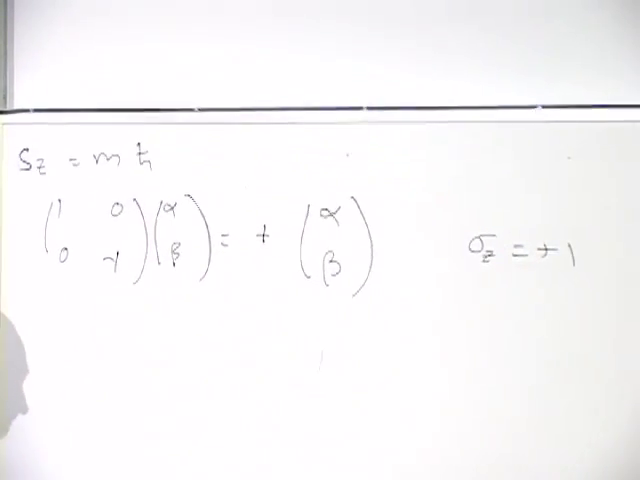
\includegraphics[width=0.74\textwidth]{lecture_08_figure_02.png}\caption{\(+1\) 고유값에 대한 \(\sigma_z\)의 고유값 방정식을 2성분 스피너에 작용시킨 결과.}\lectureframe{00:34:57}\end{figure}

고윳값이 \(+1\)인 경우, 행별로 곱하면 다음을 얻는다.
\begin{equation}
\begin{pmatrix}
1\cdot\alpha+0\cdot\beta\\
0\cdot\alpha-\beta
\end{pmatrix}
=
\begin{pmatrix}
\alpha\\
-\beta
\end{pmatrix}
=
\begin{pmatrix}
\alpha\\
\beta
\end{pmatrix}.
\end{equation}
윗줄 방정식은 자동으로 만족되고, 아랫줄에서 \(-\beta=\beta\)가 나오므로 \(\beta=0\)이다. 정규화 조건은 \(|\alpha|=1\)이다. 중요하지 않은 전체 위상을 \(\alpha=1\)가 되도록 택하면,
\begin{equation}
|+z\rangle=
\begin{pmatrix}
1\\
0
\end{pmatrix}.
\end{equation}

고윳값이 \(-1\)인 경우에는,
\begin{equation}
\begin{pmatrix}
\alpha\\
-\beta
\end{pmatrix}
=
\begin{pmatrix}
-\alpha\\
-\beta
\end{pmatrix}.
\end{equation}
이번에는 아랫줄 방정식이 자동으로 만족되고, 윗줄에서 \(\alpha=-\alpha\)가 나오므로 \(\alpha=0\)이다. \(\beta=1\)로 택하면 다음을 얻는다.
\begin{equation}
|-z\rangle=
\begin{pmatrix}
0\\
1
\end{pmatrix}.
\end{equation}

이제 실험을 바꾸어 \(S_x\)를 측정하자. 다음 관계로부터
\begin{equation}
\sigma_x
\begin{pmatrix}
\alpha\\
\beta
\end{pmatrix}
=
\begin{pmatrix}
0\cdot\alpha+\beta\\
\alpha+0\cdot\beta
\end{pmatrix}
=
\begin{pmatrix}
\beta\\
\alpha
\end{pmatrix},
\end{equation}
\(+1\) 고윳값 방정식은 다음과 같이 된다.
\begin{equation}
\begin{pmatrix}
\beta\\
\alpha
\end{pmatrix}
=
\begin{pmatrix}
\alpha\\
\beta
\end{pmatrix}.
\end{equation}
두 성분 방정식 \(\beta=\alpha\)과 \(\alpha=\beta\)은 같은 조건이다. 정규화하면
\begin{equation}
2|\alpha|^2=1,
\end{equation}
따라서 다음과 같이 택하면 편리하다.
\begin{equation}
|+x\rangle
=
\frac{1}{\sqrt2}
\begin{pmatrix}
1\\
1
\end{pmatrix}.
\end{equation}

\begin{figure}[t]\centering
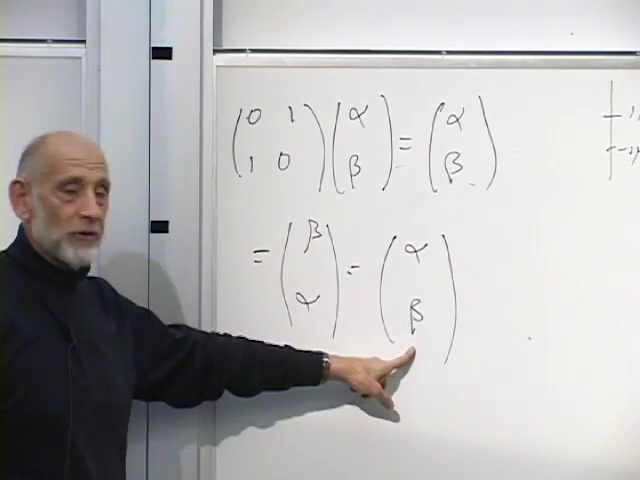
\includegraphics[width=0.74\textwidth]{lecture_08_figure_03.png}\caption{\(+1\) 고유값에서는 \(\sigma_x\)가 두 성분을 서로 바꾸므로 \(\alpha=\beta\)이어야 한다.}\lectureframe{00:39:42}\end{figure}

\begin{classroomqa}
\lecturetimestamp{00:40:13}
\audiencequestion{1/2 인자를 포함하면 고유값도 1/2이 되는가?}
\lecturerresponse{그렇다. 파울리 행렬 \(\sigma_x\)의 고유값은 \(\pm1\)이고, \(S_x=\sigma_x/2\)의 고유값은 \(\pm\tfrac12\)이다.}
\end{classroomqa}

고윳값이 \(-1\)인 경우에는,
\begin{equation}
\begin{pmatrix}
\beta\\
\alpha
\end{pmatrix}
=
-
\begin{pmatrix}
\alpha\\
\beta
\end{pmatrix},
\end{equation}
따라서
\begin{equation}
\beta=-\alpha,
\qquad
\alpha=-\beta.
\end{equation}
이 두 식은 다시 같은 방정식이다. 정규화하면
\begin{equation}
|-x\rangle
=
\frac{1}{\sqrt2}
\begin{pmatrix}
1\\
-1
\end{pmatrix}.
\end{equation}
그러므로 \(z\) 방향 스핀 업 상태와 \(z\) 방향 스핀 다운 상태를 같은 크기로 중첩하면 양의 \(x\)축 방향으로 편극되고, 상대 부호만 마이너스로 바꾸면 음의 \(x\)축 방향으로 편극된다.

\(y\) 방향의 경우,
\begin{equation}
\sigma_y
\begin{pmatrix}
\alpha\\
\beta
\end{pmatrix}
=
\begin{pmatrix}
-i\beta\\
i\alpha
\end{pmatrix}.
\end{equation}
정규화된 두 고유벡터는 다음과 같다.
\begin{equation}
|+y\rangle
=
\frac{1}{\sqrt2}
\begin{pmatrix}
1\\
i
\end{pmatrix},
\qquad
|-y\rangle
=
\frac{1}{\sqrt2}
\begin{pmatrix}
1\\
-i
\end{pmatrix},
\end{equation}
전체 위상은 임의로 정할 수 있다. 두 상태 모두 \(z\) 방향 스핀 업일 확률은 \(1/2\)이고, \(z\) 방향 스핀 다운일 확률은 \(1/2\)이다. 이 두 확률로는 알 수 없는 상대 위상 \(i\)이 \(y\) 편극과 \(x\) 편극을 구별한다. 선형 결합으로 임의의 방향으로 편극된 스핀도 나타낼 수 있지만, 그 계산은 뒤로 미룬다.

\begin{classroomqa}
\lecturetimestamp{00:44:22}
\audiencequestion{\(i\) 성분의 부호가 잘못된 \(\sigma_y\) 고유값에 배정되었는가?}
\lecturerresponse{실제로 그 부호가 잘못된 고유값에 배정되었을 수 있다. 여기서는 어느 쪽에 배정되는지 확실하지 않으며, 기억에 의존해 정하지 않는다.}
\end{classroomqa}

직접 확인하면 다음과 같다.
\begin{align}
\sigma_y\frac{1}{\sqrt2}
\begin{pmatrix}
1\\
i
\end{pmatrix}
&=
\frac{1}{\sqrt2}
\begin{pmatrix}
-i\,i\\
i
\end{pmatrix}
=
\frac{1}{\sqrt2}
\begin{pmatrix}
1\\
i
\end{pmatrix},\\
\sigma_y\frac{1}{\sqrt2}
\begin{pmatrix}
1\\
-i
\end{pmatrix}
&=
\frac{1}{\sqrt2}
\begin{pmatrix}
(-i)(-i)\\
i
\end{pmatrix}
=
-\frac{1}{\sqrt2}
\begin{pmatrix}
1\\
-i
\end{pmatrix}.
\end{align}
따라서 \(+i\)는 고유값 \(+1\)에 속하고, \(-i\)는 고유값 \(-1\)에 속한다.\footnote{말로 제시된 배정은 여러 차례 번복된 뒤에도 확정되지 않았다. 여기 표시한 부호는 행렬을 직접 곱한 결과로 정해진다.} 임의의 방향으로 편극된 상태를 포함해 모든 스핀 1/2 상태는 \(|+z\rangle\)와 \(|-z\rangle\)의 선형결합이다.

\section{스핀 1과 위치 의존 스피너}

스핀 \(1\)에서 가능한 \(S_z\) 값은 \(+1,0,-1\)이다. 따라서 상태 공간은 3차원이다. 스핀 \(1\)은 정수 스핀이며 보손 통계에 해당한다. 같은 각운동량 교환 관계를 만족하는 세 개의 \(3\times3\) 행렬을 구하자.

세 좌표 방향을 대칭적으로 다루는 표현을 아래에 제시한다.\footnote{\(S_y\)의 부호는 \(00{:}48{:}50\) 부근에 보이는 행렬에 따르며, \([S_x,S_y]=iS_z\)에 의해서도 정해진다. 그 부호를 뒤집으면 필요한 교환자의 부호도 반대로 바뀐다.}
\begin{equation}
\begin{aligned}
S_x
&=
i
\begin{pmatrix}
0&0&0\\
0&0&1\\
0&-1&0
\end{pmatrix},
&
S_y
&=
i
\begin{pmatrix}
0&0&1\\
0&0&0\\
-1&0&0
\end{pmatrix},\\
S_z
&=
i
\begin{pmatrix}
0&1&0\\
-1&0&0\\
0&0&0
\end{pmatrix}.
\end{aligned}
\end{equation}
각 행렬은 실수 반대칭 행렬에 \(i\)를 곱한 것이다. 각 행렬에는 \(1\) 하나와 \(-1\) 하나가 있으며, 해당 좌표에 대응하는 행과 열은 0이다. 첫 번째 행렬은 \(S_x\), 두 번째 행렬은 \(S_y\), 세 번째 행렬은 \(S_z\)에 대응한다. 이는 유용한 기억법이다. 이 표현에서 \(S_z\)는 대각행렬이 아니다.

다음과 같이 두자.
\begin{equation}
v=
\begin{pmatrix}
\alpha\\
\beta\\
\gamma
\end{pmatrix}.
\end{equation}
그러면
\begin{equation}
S_zv
=
\begin{pmatrix}
i\beta\\
-i\alpha\\
0
\end{pmatrix}.
\end{equation}
고윳값이 \(+1\)인 경우,
\begin{equation}
i\beta=\alpha,
\qquad
-i\alpha=\beta,
\qquad
0=\gamma.
\end{equation}
따라서 \(\beta=-i\alpha\)이고 \(\gamma=0\)이다. 정규화 조건에서 \(2|\alpha|^2=1\)이므로,
\begin{equation}
|m=+1\rangle
=
\frac{1}{\sqrt2}
\begin{pmatrix}
1\\
-i\\
0
\end{pmatrix}.
\end{equation}
고윳값이 \(-1\)인 경우에는,
\begin{equation}
i\beta=-\alpha,
\qquad
-i\alpha=-\beta,
\qquad
0=-\gamma,
\end{equation}
따라서 \(\beta=i\alpha\), \(\gamma=0\)이고,
\begin{equation}
|m=-1\rangle
=
\frac{1}{\sqrt2}
\begin{pmatrix}
1\\
i\\
0
\end{pmatrix}.
\end{equation}
마지막으로 고윳값이 0인 방정식은 \(\alpha=\beta=0\)을 주므로 \(\gamma\)은 임의로 정할 수 있다. 이를 정규화한 해는 다음과 같다.
\begin{equation}
|m=0\rangle
=
\begin{pmatrix}
0\\
0\\
1
\end{pmatrix}.
\end{equation}
세 고유벡터가 3차원 공간 전체를 이루므로 더 이상의 고윳값은 없다. 계수 \(1/\sqrt2\)는 장식이 아니다. 나중에 이 대수를 아이소스핀에 적용하면 같은 계수가 정량적인 실험 예측에 들어간다.

\begin{classroomqa}
\lecturetimestamp{00:54:10}
\audiencequestion{스핀 1 고유벡터의 복소 성분은 어떻게 읽어야 하는가?}
\lecturerresponse{\(m=+1\)의 성분은 \(1/\sqrt2,-i/\sqrt2,0\)이고, \(m=-1\)의 성분은 \(1/\sqrt2,i/\sqrt2,0\)이며, \(m=0\)의 성분은 \(0,0,1\)이다.}
\end{classroomqa}

다른 세 행렬 조합도 같은 대수를 만족하며 물리적으로 동등하다. 위의 대칭 표현은 세 방향을 똑같이 다루므로 유용하며, 뒤에서도 다시 사용한다.

\subsection{위치 자유도 되살리기}

이제 입자의 운동을 다시 고려하자. 스핀은 위치 및 운동량과 각각 교환하므로, 스핀 성분과 위치 또는 운동량을 함께 지정할 수 있다. 위치와 운동량은 서로 교환하지 않으며, 스핀 성분들도 서로 교환하지 않는다.

움직이는 스핀 1/2 입자는 위치에 따라 달라지는 스피너로 기술된다.
\begin{equation}
\psi(x)=
\begin{pmatrix}
\psi_\uparrow(x)\\
\psi_\downarrow(x)
\end{pmatrix}.
\end{equation}
다음 양들은
\begin{equation}
\rho_{\uparrow_z}(x)=|\psi_\uparrow(x)|^2,
\qquad
\rho_{\downarrow_z}(x)=|\psi_\downarrow(x)|^2
\end{equation}
위치와 스핀에 대한 결합 확률밀도다. 이들을 더하면
\begin{equation}
\rho(x)=\psi^\dagger(x)\psi(x)
=|\psi_\uparrow(x)|^2+|\psi_\downarrow(x)|^2,
\end{equation}
위치 확률밀도가 된다. 입자가 \(x\)에서 검출되었다고 알려진 경우 조건부 확률은 다음과 같다.
\begin{equation}
P(\uparrow_z\mid x)
=
\frac{|\psi_\uparrow(x)|^2}{\psi^\dagger(x)\psi(x)},
\qquad
P(\downarrow_z\mid x)
=
\frac{|\psi_\downarrow(x)|^2}{\psi^\dagger(x)\psi(x)},
\end{equation}
\(\rho(x)\neq0\)일 때 성립한다. 따라서 전자는 공간에 따라 국소 스핀 진폭이 달라질 수 있는 2성분 공간 파동함수로 표현된다.

움직이는 스핀 1 입자에 대해서는 다음과 같이 쓰자.
\begin{equation}
\phi(x)=
\begin{pmatrix}
\phi_1(x)\\
\phi_2(x)\\
\phi_3(x)
\end{pmatrix}.
\end{equation}
공간의 모든 점에서 세 성분은 앞서 사용한 것과 같은 스핀 공간의 벡터를 이룬다. 스핀 1 입자는 정수 스핀을 가지며 보손이다.

\begin{classroomqa}
\lecturetimestamp{01:00:10}
\audiencequestion{\(\phi_1(x)\) 자체가 스핀 1 결과 \(m=+1\)이 나올 확률인가?}
\lecturerresponse{아니다. 이는 선택한 3성분 기저에서의 진폭이다. 특정 스핀 결과를 얻으려면 해당하는 정규화 고유벡터의 브라를 만들고, 파동함수에 사영한 다음 절댓값 제곱을 취해야 한다.}
\end{classroomqa}

\begin{figure}[t]\centering
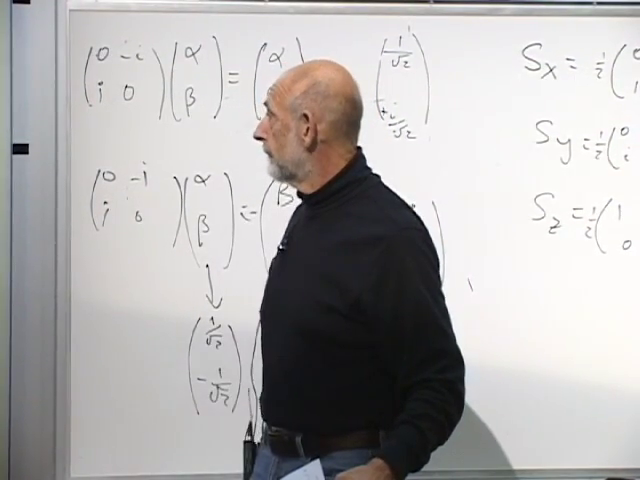
\includegraphics[width=0.82\textwidth]{lecture_08_figure_04.png}\caption{\(\sigma_y\) 정규화 고유벡터와 세 개의 스핀 1/2 행렬.}\lectureframe{01:00:12}\end{figure}

예를 들어,
\begin{equation}
\begin{aligned}
|m=+1\rangle
&=
\frac{1}{\sqrt2}
\begin{pmatrix}
1\\
-i\\
0
\end{pmatrix}
\\
\Longrightarrow\quad\langle m=+1|
&=
\frac{1}{\sqrt2}
\begin{pmatrix}
1&i&0
\end{pmatrix}.
\end{aligned}
\end{equation}
따라서 사영 진폭은
\begin{align}
\langle m=+1|\phi(x)\rangle
&=
\frac{1}{\sqrt2}
\begin{pmatrix}
1&i&0
\end{pmatrix}
\begin{pmatrix}
\phi_1(x)\\
\phi_2(x)\\
\phi_3(x)
\end{pmatrix}\\
&=
\frac{\phi_1(x)+i\phi_2(x)}{\sqrt2}.
\end{align}
같은 규칙을 세 고유벡터 모두에 적용하면 스핀별 밀도를 얻는다.\footnote{이 식들은 \(\phi_1\)와 \(\phi_2\)가 실수일 필요가 없다는 명시적인 정정을 거쳐 사영 대수를 완성한다. 이들을 실수로 취급하면 \(m=+1\) 밀도와 \(m=-1\) 밀도를 구별하는 간섭 효과가 잘못 사라진다.}
\begin{align}
\rho_{+1}(x)
&=
\frac12\left|\phi_1(x)+i\phi_2(x)\right|^2,\\
\rho_{-1}(x)
&=
\frac12\left|\phi_1(x)-i\phi_2(x)\right|^2,\\
\rho_0(x)
&=
|\phi_3(x)|^2.
\end{align}
이들은 다음 관계를 만족한다.
\begin{equation}
\begin{aligned}
\rho_{+1}(x)+\rho_{-1}(x)+\rho_0(x)
&=
|\phi_1(x)|^2+|\phi_2(x)|^2
\\
&\quad{}+|\phi_3(x)|^2
\\
&=
\phi^\dagger(x)\phi(x).
\end{aligned}
\end{equation}
입자가 \(x\)에서 검출되었다고 조건을 걸면,
\begin{equation}
P(m\mid x)
=
\frac{\rho_m(x)}{\phi^\dagger(x)\phi(x)},
\end{equation}
\(\phi^\dagger(x)\phi(x)\neq0\)인 경우에 성립한다. 일반적인 측정 규칙은 늘 같다. 원하는 정규화 고유벡터의 브라를 만들고, 실제 상태를 그 벡터에 사영한 뒤 절댓값을 제곱한다. 이렇게 얻은 밀도에는 위치 의존성이 그대로 남는다.

스핀이 높아지면 행렬은 더 복잡해지지만 원리는 달라지지 않는다.

\begin{classroomqa}
\lecturetimestamp{01:07:31}
\audiencequestion{스핀 3/2의 상태 공간 차원은 얼마인가?}
\lecturerresponse{상태는 네 개이며, \(m=\tfrac32,\tfrac12,-\tfrac12,-\tfrac32\)이다. 스핀 2에는 상태가 다섯 개 있다.}
\end{classroomqa}

\begin{classroomqa}
\lecturetimestamp{01:07:55}
\audiencequestion{\(x,y,z\)는 다루면서 시간 방향은 다루지 않은 이유는 무엇인가? 이 설명은 비상대론적인가?}
\lecturerresponse{지금까지는 비상대론적이다. 질량과 마찬가지로 스핀도 입자의 정지계에서 가장 간단히 특성화할 수 있다. 다른 관성계에서의 기술은 적절한 로런츠 변환으로 얻는다. 이 상대론적 단계는 뒤에서 다룬다.}
\end{classroomqa}

디랙 방정식은 상대론적 틀을 제공하며, 디랙 파동함수가 네 성분을 가지면서 스핀 이중항을 포함하는 이유를 설명한다.

\section{디랙 행렬과 4성분 스피너}

4성분 디랙 파동함수는 다음을 만족한다.
\begin{equation}
i\frac{\partial\Psi}{\partial t}
=
-i\alpha_i\frac{\partial\Psi}{\partial x_i}
+m\beta\Psi,
\qquad i=1,2,3,
\end{equation}
여기서는 반복된 공간 첨자에 대해 합한다. 따라서 미분 항은 다음을 뜻한다.
\begin{equation}
\alpha_1\frac{\partial\Psi}{\partial x}
+\alpha_2\frac{\partial\Psi}{\partial y}
+\alpha_3\frac{\partial\Psi}{\partial z}.
\end{equation}
평면파의 경우 이는 대수 방정식이 된다.
\begin{equation}
\omega\Psi=(\alpha_i k_i+m\beta)\Psi.
\end{equation}

\begin{classroomqa}
\lecturetimestamp{01:11:32}
\audiencequestion{\(m\)가 두 번 나올 때 두 기호는 같은 것을 뜻하는가?}
\lecturerresponse{아니다. 하나는 공간 첨자로 쓰였고, 다른 하나는 입자의 질량이다. 공간 첨자를 \(i\)로 바꾸자. \(i\)가 두 번 나오면 \(1\)부터 \(3\)까지 합한다.}
\end{classroomqa}

진동수 연산자를 제곱하면 상대론적 관계식이 재현되어야 한다.
\begin{equation}
\omega^2=\mathbf{k}^2+m^2.
\end{equation}
따라서 제곱 항으로부터 각 \(i\)에 대해 다음이 요구된다.
\begin{equation}
\alpha_i^2=I_4,
\qquad
\beta^2=I_4.
\end{equation}

\begin{classroomqa}
\lecturetimestamp{01:13:01}
\audiencequestion{\(\beta\)는 \(\Psi\)의 네 성분마다 서로 다른가?}
\lecturerresponse{아니다. 네 성분 스피너 전체에 작용하는 행렬 \(\beta\) 하나가 있으며, 이 행렬은 \(\beta^2=I_4\)를 만족한다.}
\end{classroomqa}

혼합항은 0이어야 한다. 서로 다른 공간 방향 사이뿐 아니라 각 \(\alpha_i\)와 \(\beta\) 사이에서도 다음이 성립한다.
\begin{equation}
\alpha_i\alpha_j+\alpha_j\alpha_i=0
\quad (i\neq j),
\qquad
\alpha_i\beta+\beta\alpha_i=0.
\end{equation}
이를 동등하게 쓰면 다음과 같다.
\begin{equation}
\{\alpha_i,\alpha_j\}=2\delta_{ij}I_4,
\quad
\{\alpha_i,\beta\}=0,
\quad
\{\beta,\beta\}=2I_4.
\end{equation}
각 행렬은 자신과 다른 모든 행렬과 반교환하며, 자기 자신과의 반교환자는 단위행렬의 두 배다.

\(\beta\)를 제외하면 세 파울리 행렬은 이미 항등 행렬로 제곱되고 서로 반교환하는 세 개의 \(2\times2\) 행렬을 제공한다. 질량 항을 위해서는 이 성질을 갖는 네 번째 행렬이 필요하다. 필요한 성질을 만족하는 네 번째 \(2\times2\) 행렬은 없으며, \(3\times3\) 행렬로도 이 대수를 만족시킬 수 없다. 따라서 최소 표현은 \(4\times4\)이다.

\(4\times4\) 행렬은 네 개의 \(2\times2\) 블록으로 나눌 수 있다. 편리한 표현 하나는 다음과 같다.
\begin{equation}
\alpha_i=
\begin{pmatrix}
\sigma_i&0\\
0&-\sigma_i
\end{pmatrix},
\qquad i=1,2,3.
\end{equation}

\begin{figure}[t]\centering
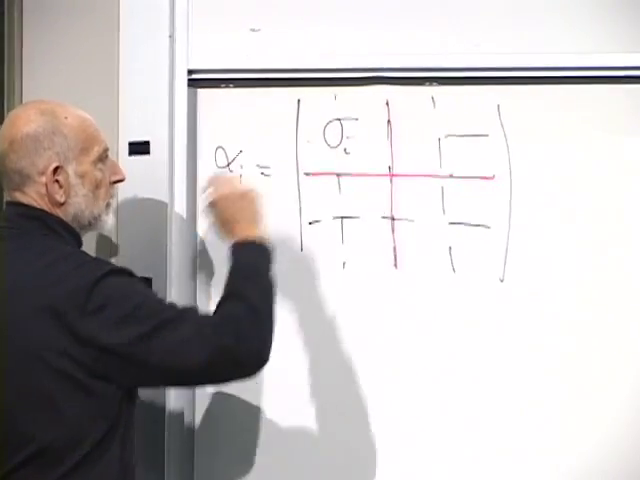
\includegraphics[width=0.68\textwidth]{lecture_08_figure_05.png}\caption{\(\alpha_i\) 디랙 행렬을 \(2\times2\) 블록으로 나타낸 것. 대각 블록은 \(\sigma_i\)와 \(-\sigma_i\)이다.}\lectureframe{01:17:23}\end{figure}

\begin{classroomqa}
\lecturetimestamp{01:17:41}
\audiencequestion{앞선 표현에서는 \(\sigma_i\) 블록이 반대 방식으로 배열되어 있었는가?}
\lecturerresponse{그렇다. 다른 표현에서는 대각선이 아닌 위치에 놓였다. 두 배열은 동등하며 닮음 변환으로 서로 연결된다.}
\end{classroomqa}

현재 표현에서 나머지 행렬은 다음과 같다.
\begin{equation}
\beta=
\begin{pmatrix}
0&I_2\\
I_2&0
\end{pmatrix},
\qquad
I_2=
\begin{pmatrix}
1&0\\
0&1
\end{pmatrix}.
\end{equation}
블록 곱셈을 이용하면 \(4\times4\) 대수의 검산을 보통의 \(2\times2\) 행렬 곱셈으로 줄일 수 있다.

\begin{classroomqa}
\lecturetimestamp{01:19:17}
\audiencequestion{앞선 표현에서 \(\beta\)는 부호가 달랐거나 대각 형태였는가?}
\lecturerresponse{앞선 표현에서는 다르지만 물리적으로 동등한 기저를 사용했다. 기저를 바꾸면 \(\Psi\)의 네 성분이 서로 섞이고 행렬의 모양도 달라지지만, 물리는 변하지 않는다.}
\end{classroomqa}

\(\Psi\)의 네 성분은 시공간의 네 좌표가 아니다. 이 성분들은 반교환 대수가 작용할 수 있는 가장 작은 벡터 공간의 좌표다. 여기에는 서로 다른 두 가지 이중 구조가 있다. \(2\times2\) 블록으로 나뉘고, 각 블록 안에는 2성분 파울리 구조가 있다. 아래에서 확립할 해석을 미리 적용하면 네 가지 경우를 다음과 같이 배열할 수 있다.
\begin{equation}
\begin{array}{c|cc}
& S_z=+\tfrac12 & S_z=-\tfrac12\\ \hline
\omega>0 & (\omega>0,+\tfrac12) & (\omega>0,-\tfrac12)\\
\omega<0 & (\omega<0,+\tfrac12) & (\omega<0,-\tfrac12)
\end{array}.
\end{equation}
아랫줄은 음의 진동수를 갖는 전자 상태들이다. 양전자 행이 아니다. 양전자는 이 상태들의 채워진 집합에 생긴 구멍으로 해석할 것이다.

\section{정지계 에너지 이중성과 양전자}

운동량이 0일 때 에너지의 이중 구조가 가장 쉽게 드러난다. \(\mathbf{k}=0\)이면 평면파 상태는 공간적으로 일정하고 공간 미분 항은 사라진다. 정지계 방정식\footnote{\(01{:}23{:}38\)에서 질량 항에 일시적으로 추가 인자 \(i\)가 붙어 있지만, \(01{:}24{:}05\)에서 구술 중 정정해 이를 제거했다.}은 다음과 같다.
\begin{equation}
i\frac{\partial\Psi}{\partial t}=m\beta\Psi.
\end{equation}

\begin{figure}[t]\centering
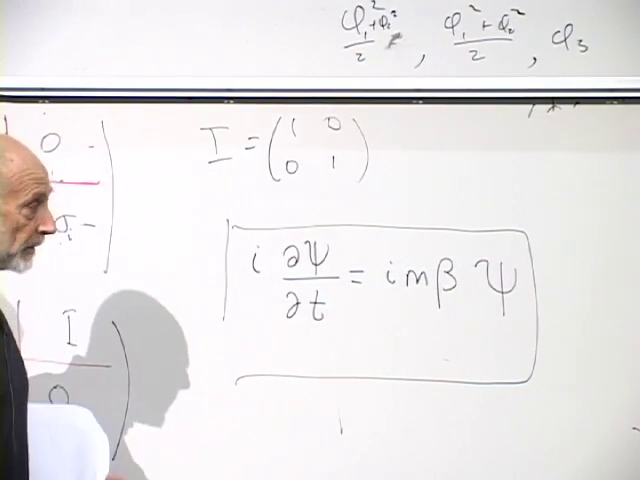
\includegraphics[width=0.76\textwidth]{lecture_08_figure_06.png}\caption{운동량이 0이면 공간 미분항은 사라지고, 보정된 정지계 방정식 \(i\partial_t\Psi=m\beta\Psi\)만 남는다.}\lectureframe{01:23:38}\end{figure}

4성분 열벡터를 위쪽과 아래쪽의 2성분 객체로 나누어 쓰자.
\begin{equation}
\Psi=
\begin{pmatrix}
\psi_+\\
\psi_-
\end{pmatrix}.
\end{equation}

\begin{classroomqa}
\lecturetimestamp{01:24:47}
\audiencequestion{\(\psi_+\)와 \(\psi_-\)라는 표기는 이미 양에너지와 음에너지를 뜻합니까?}
\lecturerresponse{아닙니다. 이 단계에서는 위쪽과 아래쪽의 두 성분 블록을 가리키는 이름일 뿐입니다. 각 블록에 해당하는 에너지 조합은 아직 구하지 않았습니다.}
\end{classroomqa}

\begin{classroomqa}
\lecturetimestamp{01:25:10}
\audiencequestion{나누어 쓴 4성분 열은 무엇을 나타냅니까?}
\lecturerresponse{행렬의 블록 형태에 맞춰 정리한 동일한 4성분 디랙 스피너입니다. 각 절반은 2성분 객체이며, 이런 객체 두 개가 원래의 4성분 열을 이룹니다.}
\end{classroomqa}

행렬 \(\beta\)는 두 블록을 서로 바꿉니다.
\begin{equation}
\beta
\begin{pmatrix}
\psi_+\\
\psi_-
\end{pmatrix}
=
\begin{pmatrix}
\psi_-\\
\psi_+
\end{pmatrix}.
\end{equation}
따라서 정지계 방정식은 다음과 같이 됩니다.
\begin{equation}
i\frac{\partial\psi_+}{\partial t}=m\psi_-,
\qquad
i\frac{\partial\psi_-}{\partial t}=m\psi_+.
\end{equation}

자연스러운 방법은 두 가지입니다. 시간에 대해 한 번 더 미분하면 연립방정식을 분리할 수 있지만, 두 방정식을 더하고 빼면 곧바로 대각화됩니다. 실제로,
\begin{align}
i\frac{\partial}{\partial t}(\psi_++\psi_-)
&=m(\psi_++\psi_-),\\
i\frac{\partial}{\partial t}(\psi_+-\psi_-)
&=-m(\psi_+-\psi_-).
\end{align}
다음과 같이 정의하면
\begin{equation}
\chi_+=\psi_++\psi_-,
\qquad
\chi_-=\psi_+-\psi_-,
\end{equation}
서로 독립인 두 방정식을 얻습니다.
\begin{equation}
i\partial_t\chi_+=m\chi_+,
\qquad
i\partial_t\chi_-=-m\chi_-.
\end{equation}
주파수가 정해진 의존성 \(e^{-i\omega t}\)을 가정하면, 합에 대해서는
\begin{equation}
\omega=+m,
\end{equation}
차에 대해서는
\begin{equation}
\omega=-m.
\end{equation}
를 얻습니다. 이는 앞서 살펴본 1차원 예에서 나타난 양에너지와 음에너지의 이중성과 정확히 같습니다. 상대론적 방정식에는 다시 양에너지 전자 해와 음에너지 전자 해가 존재합니다. 따라서 블록의 이중성은 양에너지 가지와 음에너지 가지로 나뉩니다. 정지계의 순수 상태는 다음과 같이 쓸 수 있습니다.
\begin{equation}
\Psi_{\omega=+m}=
\begin{pmatrix}
\xi\\
\xi
\end{pmatrix},
\qquad
\Psi_{\omega=-m}=
\begin{pmatrix}
\xi\\
-\xi
\end{pmatrix},
\end{equation}
여기서 \(\xi\)는 여전히 임의의 2성분 객체입니다.

합과 차를 취하면 두 겹 구조 가운데 하나는 정리되지만, \(\xi\)의 두 성분은 여전히 남습니다. 파울리 행렬은 이 남은 두 성분에 작용합니다. 이 성분 쌍은 스핀과 관련된 것으로, 아래에서 다룰 회전 및 보존 법칙 검증을 거쳐야 합니다.

\begin{classroomqa}
\lecturetimestamp{01:32:23}
\audiencequestion{스핀을 바깥쪽의 두 겹 구조로, 에너지 부호를 안쪽 구조로 볼 수 있습니까?}
\lecturerresponse{네. 두 인자의 순서는 서로 바꾸어도 동등합니다. 어느 지표를 먼저 쓸지 바꿀 수 있으며, 달라지는 것은 네 성분의 배열뿐입니다.}
\end{classroomqa}

음의 주파수 가지는 디랙 바다 해석으로 이어집니다. 음의 주파수에는 음의 전자 에너지를 대응시킵니다. 배타 원리에 따라 완전한 페르미온 상태 하나에는 전자 하나만 들어갈 수 있으므로, 허용되는 한 모든 음에너지 전자 상태를 채우면 에너지가 낮아집니다. 이렇게 음에너지 상태를 완전히 채운 바다를 진공이라고 부릅니다.

이 채워진 바다에서 전자 하나를 양에너지 상태로 끌어올려 보겠습니다. 그러면 양에너지 전자 하나와 비어 있는 음에너지 상태 하나가 남습니다. 음의 에너지를 제거하면 에너지가 증가하므로, 이 구멍은 양의 여기 에너지를 가집니다. 전자가 하나 빠져 있으므로 전하도 반대 부호입니다. 이 구멍이 양전자입니다.

\begin{classroomqa}
\lecturetimestamp{01:32:57}
\audiencequestion{양전자를 해석하는 방법을 다시 설명해 주시겠습니까?}
\lecturerresponse{두 블록의 합은 양의 주파수를, 차는 음의 주파수를 가집니다. 음의 주파수 해는 음에너지 전자 상태이며, 그 상태를 모두 채우면 진공이 됩니다. 채워진 상태의 전자 하나를 양에너지로 끌어올리면 양에너지 전자와 구멍이 함께 남습니다. 양의 에너지를 가지면서 전하가 반대인 이 구멍이 양전자입니다.}
\end{classroomqa}

따라서 이 대수적 구성에서는 두 가지 결과가 동시에 나옵니다. 양에너지와 음에너지 가지는 입자--반입자 구조로 이어지고, 남은 2성분 구조는 스핀 1/2와 관련됩니다. 놀라운 점은 상대론적 반교환 관계를 만족하는 최소 행렬에서 이 두 결과가 모두 나왔다는 것입니다. 당시 스핀은 실험적으로 알려진 지 얼마 되지 않은 성질이었는데, 이 수학적 구성에서 스핀을 가진 입자와 반입자 가지가 함께 나타났습니다. 당시의 맥락에서 이는 극적인 결과였습니다.

\begin{classroomqa}
\lecturetimestamp{01:35:14}
\audiencequestion{음에너지 전자 자체가 양전자입니까?}
\lecturerresponse{아닙니다. 음에너지 전자 상태는 진공에서 채워져 있습니다. 양전자는 그 채워진 상태들 가운데 전자 하나가 빠진 경우, 즉 구멍이지 음에너지 전자가 아닙니다.}
\end{classroomqa}

구멍은 전이 과정에 참여할 수 있습니다. 양전자가 양의 에너지를 갖는 까닭은 음에너지 전자가 하나 없는 상태이기 때문입니다. 양에너지 전자가 그 구멍을 채우면 전자와 양전자는 소멸하지만, 에너지는 보통 광자의 형태로 빠져나가야 합니다. 바다의 관점에서 보면 전자가 비어 있던 음에너지 상태를 채운 것입니다. 같은 에너지 방출을 원자 안의 여기된 전자가 더 낮은 준위로 내려가는 과정으로 나타낼 수도 있습니다. 아래쪽으로 전이하면서 광자를 방출합니다.

\begin{classroomqa}
\lecturetimestamp{01:36:39}
\audiencequestion{더 높은 음에너지 전자는 왜 구멍으로 떨어지지 않습니까?}
\lecturerresponse{이 질문은 서로 다른 두 경우를 혼동하고 있습니다. 양에너지 전자가 구멍을 채우는 것은 전자--양전자 소멸이며, 광자가 에너지를 가져갑니다. 음에너지 바다의 전자가 전이하는 과정은 다른 과정으로, 아래에서 다룹니다.}
\end{classroomqa}

운동량이 0인 경우의 계산만으로 에너지 부호를 분리한 뒤 두 겹 축퇴가 존재한다는 점은 밝혀졌습니다. 하지만 상태가 두 개라는 축퇴만으로 그 상태들이 각운동량을 가진다고 증명되지는 않습니다.

\begin{classroomqa}
\lecturetimestamp{01:37:44}
\audiencequestion{운동량이 0인 경우의 계산은 남은 상태 쌍이 스핀이라는 것을 어떻게 증명합니까?}
\lecturerresponse{그 상태 쌍을 스핀 위와 아래라고 부를 수 있고 전체 방정식에 파울리 행렬이 나타나지만, 그것만으로는 아직 증명이 되지 않습니다. 이 상태 쌍이 공간 회전 아래에서 어떻게 변환되는지 보이거나, 상호작용과 충돌에서 스핀을 부여했을 때 총각운동량이 보존됨을 보여야 합니다. 그 증명은 뒤에서 다루겠습니다.}
\end{classroomqa}

양에너지를 가진 정지 상태에서는 위쪽 블록과 아래쪽 블록이 같습니다.
\begin{equation}
\Psi_{\omega=+m}=
\begin{pmatrix}
\xi\\
\xi
\end{pmatrix}.
\end{equation}
\(\xi\)가 각운동량 이중항임을 보이려면 앞서 말한 회전 또는 보존 법칙 논증이 필요합니다. 성분이 두 개라는 사실만으로는 이 결론이 나오지 않습니다.

\begin{classroomqa}
\lecturetimestamp{01:40:46}
\audiencequestion{에너지가 서로 달라도 다른 전자가 양전자와 소멸할 수 있습니까?}
\lecturerresponse{네. 전자는 각자 고유한 정체성을 유지하지 않습니다. 가능한 전자라면 어느 것이든 구멍을 채울 수 있으며, 초기 에너지와 운동량의 차이는 방출되는 광자의 수와 에너지에 반영됩니다.}
\end{classroomqa}

구멍의 관점으로 보면 음에너지 바다 안에서만 일어나는 전이도 설명할 수 있습니다. 음에너지 상태 하나에 있던 전자가 구멍으로 이동한다고 합시다. 원래의 구멍은 채워지지만, 전자가 있던 상태가 이제 비게 됩니다. 구멍이 이동한 것입니다. 다시 말해 양전자의 에너지가 바뀌면서 복사를 방출한 것입니다.

\begin{classroomqa}
\lecturetimestamp{01:42:12}
\audiencequestion{인접한 음에너지 준위의 전자들이 왜 차례로 구멍으로 떨어지지 않습니까?}
\lecturerresponse{전자들은 구멍을 한 준위에서 다른 준위로 옮길 수 있습니다. 전자가 기존 구멍으로 내려오면 원래 그 전자가 있던 에너지에 새 구멍이 생기므로, 처음의 양전자는 에너지가 다른 양전자가 됩니다. 에너지 차이는 광자가 가져갑니다.}
\end{classroomqa}

\begin{classroomqa}
\lecturetimestamp{01:44:39}
\audiencequestion{그렇다면 왜 복사를 내며 계속 아래로 내려가는 연쇄 과정이 생기지 않습니까?}
\lecturerresponse{에너지와 운동량이 동시에 보존되어야 하기 때문입니다. 이 두 보존 법칙 때문에 그런 과정이 제한 없이 일어날 수는 없습니다. 보통의 자유 전자도 마찬가지입니다. 빈 공간에서 광자를 방출하며 에너지를 계속 낮출 수는 없습니다.}
\end{classroomqa}
